% setup.tex - ManiSkill3 Setup Guide
% AlohaMini Robot Integration
% Standalone document

\documentclass[aspectratio=169]{beamer}

% Theme settings
\usetheme{CambridgeUS}
\usecolortheme{default}

% Define darkred color for compatibility
\definecolor{darkred}{rgb}{0.55, 0.0, 0.0}

% Load common preamble
% AlohaMini Documentation - Common Preamble
% Beamer presentation with beaver theme

% ============================================
% PACKAGES
% ============================================

% TikZ for diagrams
\usepackage{tikz}
\usetikzlibrary{
    arrows.meta,
    shapes.geometric,
    shapes.misc,
    positioning,
    calc,
    fit,
    backgrounds,
    decorations.pathreplacing,
    chains
}

% Code listings
\usepackage{listings}
\usepackage{xcolor}

% Math
\usepackage{amsmath}
\usepackage{amssymb}

% Tables
\usepackage{booktabs}
\usepackage{array}
\usepackage{multirow}

% Graphics
\usepackage{graphicx}

% Hyperlinks
\usepackage{hyperref}

% Korean support (optional)
\usepackage{kotex}

% ============================================
% CODE LISTING STYLE
% ============================================

\definecolor{codegreen}{rgb}{0,0.6,0}
\definecolor{codegray}{rgb}{0.5,0.5,0.5}
\definecolor{codepurple}{rgb}{0.58,0,0.82}
\definecolor{backcolour}{rgb}{0.95,0.95,0.92}
\definecolor{codeblue}{rgb}{0.13,0.13,0.8}

\lstdefinestyle{pythonstyle}{
    backgroundcolor=\color{backcolour},
    commentstyle=\color{codegreen}\itshape,
    keywordstyle=\color{codeblue}\bfseries,
    numberstyle=\tiny\color{codegray},
    stringstyle=\color{codepurple},
    basicstyle=\ttfamily\tiny,
    breakatwhitespace=false,
    breaklines=true,
    captionpos=b,
    keepspaces=true,
    numbers=left,
    numbersep=3pt,
    showspaces=false,
    showstringspaces=false,
    showtabs=false,
    tabsize=2,
    language=Python,
    morekeywords={self, True, False, None, def, class, return, import, from, as, if, else, elif, for, while, try, except, finally, with, yield, lambda, and, or, not, in, is, pass, break, continue, raise, assert, global, nonlocal, async, await},
    frame=single,
    framerule=0.5pt,
    rulecolor=\color{codegray}
}

\lstset{style=pythonstyle}

% Inline code
\newcommand{\code}[1]{\texttt{\small #1}}
\newcommand{\pycode}[1]{\lstinline[language=Python]{#1}}

% ============================================
% TIKZ STYLES
% ============================================

\tikzstyle{module} = [
    rectangle,
    rounded corners=3pt,
    draw=darkred!80,
    fill=darkred!10,
    text width=2.5cm,
    minimum height=1cm,
    text centered,
    font=\small\bfseries
]

\tikzstyle{submodule} = [
    rectangle,
    rounded corners=2pt,
    draw=gray!60,
    fill=gray!10,
    text width=2cm,
    minimum height=0.7cm,
    text centered,
    font=\footnotesize
]

\tikzstyle{class} = [
    rectangle,
    draw=blue!60,
    fill=blue!10,
    text width=3cm,
    minimum height=0.8cm,
    text centered,
    font=\small\ttfamily
]

\tikzstyle{arrow} = [
    ->,
    >=stealth,
    thick,
    draw=darkred!70
]

\tikzstyle{flow} = [
    ->,
    >=Triangle,
    thick,
    draw=gray!70
]

\tikzstyle{joint} = [
    circle,
    draw=black,
    fill=orange!30,
    minimum size=0.4cm
]

\tikzstyle{link} = [
    line width=3pt,
    draw=gray!60
]

% ============================================
% CUSTOM COMMANDS
% ============================================

% File path styling
\newcommand{\filepath}[1]{\texttt{\color{codeblue}\small #1}}

% Highlight box
\newcommand{\highlight}[1]{%
    \colorbox{yellow!30}{\texttt{#1}}%
}

% Warning/Note boxes
\newenvironment{notebox}{%
    \begin{block}{Note}
}{%
    \end{block}
}

\newenvironment{warningbox}{%
    \begin{alertblock}{Warning}
}{%
    \end{alertblock}
}

% ============================================
% BEAMER CUSTOMIZATION
% ============================================

% Reduce text margins for more content space
\setbeamersize{text margin left=4mm, text margin right=4mm}

% Allow sloppy line breaking
\sloppy

% Tolerate small hbox/vbox overflows (up to 20pt for presentations)
\hfuzz=20pt
\vfuzz=20pt

% Frame title format (compact)
\setbeamertemplate{frametitle}{
    \vspace{0.3em}
    \insertframetitle
    \par
    \vspace{-0.4em}
    \textcolor{darkred!50}{\rule{\textwidth}{0.3pt}}
}

% Footer with page numbers
\setbeamertemplate{footline}{
    \leavevmode%
    \hbox{%
        \begin{beamercolorbox}[wd=.333333\paperwidth,ht=2.25ex,dp=1ex,left]{author in head/foot}%
            \usebeamerfont{author in head/foot}\hspace{1em}AlohaMini Documentation
        \end{beamercolorbox}%
        \begin{beamercolorbox}[wd=.333333\paperwidth,ht=2.25ex,dp=1ex,center]{title in head/foot}%
            \usebeamerfont{title in head/foot}\insertshorttitle
        \end{beamercolorbox}%
        \begin{beamercolorbox}[wd=.333333\paperwidth,ht=2.25ex,dp=1ex,right]{date in head/foot}%
            \usebeamerfont{date in head/foot}\insertframenumber{} / \inserttotalframenumber\hspace{1em}
        \end{beamercolorbox}%
    }%
    \vskip0pt%
}

% Remove navigation symbols
\setbeamertemplate{navigation symbols}{}

% Table of contents styling
\setbeamertemplate{section in toc}[sections numbered]
\setbeamertemplate{subsection in toc}[subsections numbered]


% ============================================
% DOCUMENT INFORMATION
% ============================================

\title[ManiSkill Setup]{ManiSkill3 Setup Guide}
\subtitle{AlohaMini Robot Integration}
\author{Technical Documentation}
\date{\today}
\institute{AlohaMini Project}

% ============================================
% DOCUMENT BODY
% ============================================

\begin{document}

% Title slide
\begin{frame}
    \titlepage
\end{frame}

% Table of contents
\begin{frame}{Contents}
    \tableofcontents
\end{frame}

% ============================================
% SECTION 1: OVERVIEW
% ============================================
\section{Overview}

\begin{frame}{Setup Overview}
\begin{columns}
\begin{column}{0.45\textwidth}
    \textbf{Purpose:}\\
    Integrate AlohaMini robot into ManiSkill3 simulation framework.

    \vspace{0.3cm}

    \textbf{Key Components:}
    \begin{itemize}
        \item \code{install.py} - Installation script
        \item \code{setup.py} - Package configuration
        \item Agent files (\code{*.py})
        \item URDF \& mesh assets
    \end{itemize}
\end{column}
\begin{column}{0.55\textwidth}
    \centering
    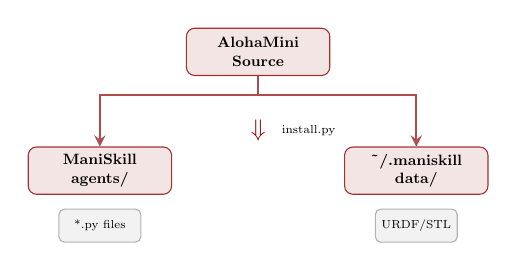
\begin{tikzpicture}[scale=0.6, transform shape, node distance=1.2cm]
        % Source
        \node[module, text width=2.8cm] (src) {AlohaMini\\Source};

        % Arrow
        \node[below=0.8cm of src] (arrow) {\Large\color{darkred}$\Downarrow$};
        \node[right=0.1cm of arrow] {\scriptsize install.py};

        % Destinations
        \node[module, text width=2.8cm, below left=1.5cm and 0.3cm of src] (agents) {ManiSkill\\agents/};
        \node[module, text width=2.8cm, below right=1.5cm and 0.3cm of src] (data) {\textasciitilde/.maniskill\\data/};

        % Arrows
        \draw[arrow] (src.south) -- ++(0,-0.4) -| (agents.north);
        \draw[arrow] (src.south) -- ++(0,-0.4) -| (data.north);

        % Labels
        \node[submodule, text width=1.5cm, below=0.3cm of agents] {\scriptsize *.py files};
        \node[submodule, text width=1.5cm, below=0.3cm of data] {\scriptsize URDF/STL};
    \end{tikzpicture}
\end{column}
\end{columns}
\end{frame}

% ============================================
% SECTION 2: PREREQUISITES
% ============================================
\section{Prerequisites}

\begin{frame}[fragile]{Prerequisites}
\begin{columns}
\begin{column}{0.5\textwidth}
    \textbf{System Requirements:}
    \begin{itemize}
        \item Python $\geq$ 3.8
        \item CUDA (for GPU acceleration)
        \item Linux / macOS / Windows
    \end{itemize}

    \vspace{0.3cm}

    \textbf{Package Dependencies:}
    \begin{itemize}
        \item \code{mani-skill >= 3.0.0b0}
        \item \code{numpy}
        \item \code{pygame} (optional, for keyboard)
    \end{itemize}
\end{column}
\begin{column}{0.5\textwidth}
\textbf{Installation Commands:}
\begin{lstlisting}[basicstyle=\ttfamily\scriptsize]
# Create virtual environment
python -m venv venv
source venv/bin/activate

# Install ManiSkill3
pip install mani-skill

# Verify installation
python -c "import mani_skill; print(mani_skill.__version__)"
\end{lstlisting}
\end{column}
\end{columns}
\end{frame}

\begin{frame}[fragile]{setup.py Configuration}
\begin{lstlisting}
from setuptools import setup, find_packages

setup(
    name="aloha_mini_maniskill",
    version="0.1.0",
    description="AlohaMini dual-arm mobile robot for ManiSkill3",
    packages=find_packages(),
    package_data={
        "aloha_mini": ["*.urdf", "meshes/*.STL"],
    },
    install_requires=[
        "mani-skill>=3.0.0b0",
        "numpy",
    ],
    extras_require={
        "dev": ["pygame"],  # For keyboard control
    },
    python_requires=">=3.8",
)
\end{lstlisting}
\end{frame}

% ============================================
% SECTION 3: INSTALLATION
% ============================================
\section{Installation}

\begin{frame}{Installation Process}
\begin{columns}
\begin{column}{0.5\textwidth}
    \textbf{4-Step Process:}
    \begin{enumerate}
        \item \textbf{Agent Files}\\
              Copy \code{*.py} to ManiSkill agents
        \item \textbf{URDF \& Meshes}\\
              Copy to \code{\textasciitilde/.maniskill/data/}
        \item \textbf{Scene Builder}\\
              Update ReplicaCAD integration
        \item \textbf{Registration}\\
              Add import to \code{\_\_init\_\_.py}
    \end{enumerate}
\end{column}
\begin{column}{0.5\textwidth}
    \centering
    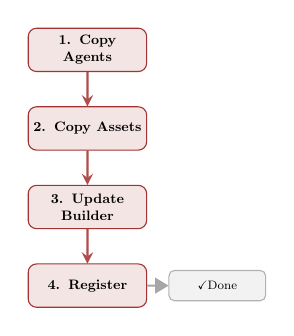
\begin{tikzpicture}[scale=0.55, transform shape, node distance=0.8cm]
        \node[module, text width=2.5cm] (step1) {1. Copy Agents};
        \node[module, text width=2.5cm, below=of step1] (step2) {2. Copy Assets};
        \node[module, text width=2.5cm, below=of step2] (step3) {3. Update Builder};
        \node[module, text width=2.5cm, below=of step3] (step4) {4. Register};

        \draw[arrow] (step1) -- (step2);
        \draw[arrow] (step2) -- (step3);
        \draw[arrow] (step3) -- (step4);

        \node[submodule, text width=2cm, right=0.5cm of step4] (done) {\checkmark Done};
        \draw[flow] (step4) -- (done);
    \end{tikzpicture}
\end{column}
\end{columns}
\end{frame}

\begin{frame}[fragile]{install.py - Path Discovery}
\begin{lstlisting}
def find_maniskill_path():
    """Find the ManiSkill installation path."""
    try:
        import mani_skill
        return Path(mani_skill.__file__).parent
    except ImportError:
        print("Error: ManiSkill not installed.")
        sys.exit(1)

def get_maniskill_data_dir():
    """Get the ManiSkill data directory."""
    return Path.home() / ".maniskill" / "data"
\end{lstlisting}

\begin{block}{Key Insight}
ManiSkill stores robot assets in \code{\textasciitilde/.maniskill/data/robots/}
\end{block}
\end{frame}

\begin{frame}[fragile]{install.py - Copy Files}
\begin{lstlisting}[basicstyle=\ttfamily\scriptsize]
def install():
    script_dir = Path(__file__).parent.resolve()
    maniskill_path = find_maniskill_path()
    data_dir = get_maniskill_data_dir()

    # 1. Install agent files
    agent_src = script_dir / "agents" / "aloha_mini"
    agent_dst = maniskill_path / "agents" / "robots" / "aloha_mini"
    agent_dst.mkdir(parents=True, exist_ok=True)
    for f in agent_src.glob("*.py"):
        shutil.copy2(f, agent_dst / f.name)

    # 2. Install URDF and mesh files
    asset_src = script_dir / "assets" / "robots" / "aloha_mini"
    asset_dst = data_dir / "robots" / "aloha_mini"
    shutil.copytree(asset_src, asset_dst)
\end{lstlisting}
\end{frame}

% ============================================
% SECTION 4: DIRECTORY STRUCTURE
% ============================================
\section{Directory Structure}

\begin{frame}{Directory Mapping}
\begin{columns}
\begin{column}{0.45\textwidth}
    \textbf{Source (AlohaMini):}
    \begin{itemize}
        \item \filepath{maniskill/agents/aloha\_mini/*.py}
        \item \filepath{maniskill/assets/robots/aloha\_mini/}
        \item \filepath{maniskill/scene\_builder/}
    \end{itemize}

    \vspace{0.3cm}

    \textbf{Destination (ManiSkill):}
    \begin{itemize}
        \item \filepath{mani\_skill/agents/robots/aloha\_mini/}
        \item \filepath{\textasciitilde/.maniskill/data/robots/aloha\_mini/}
        \item \filepath{mani\_skill/utils/scene\_builder/}
    \end{itemize}
\end{column}
\begin{column}{0.55\textwidth}
    \centering
    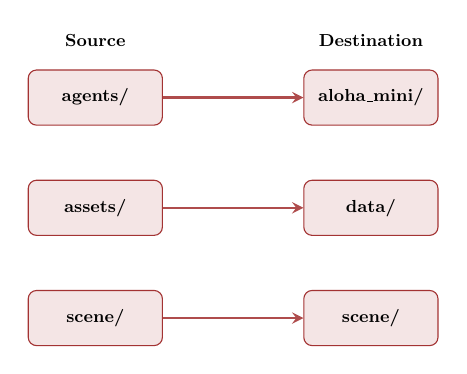
\begin{tikzpicture}[scale=0.7, transform shape]
        % Source side
        \node[module, text width=2.2cm] (src_agents) at (-2,2) {agents/};
        \node[module, text width=2.2cm] (src_assets) at (-2,0) {assets/};
        \node[module, text width=2.2cm] (src_scene) at (-2,-2) {scene/};

        % Destination side
        \node[module, text width=2.2cm] (dst_agents) at (3,2) {aloha\_mini/};
        \node[module, text width=2.2cm] (dst_assets) at (3,0) {data/};
        \node[module, text width=2.2cm] (dst_scene) at (3,-2) {scene/};

        % Arrows
        \draw[arrow] (src_agents) -- (dst_agents);
        \draw[arrow] (src_assets) -- (dst_assets);
        \draw[arrow] (src_scene) -- (dst_scene);

        % Labels
        \node[above=0.3cm of src_agents] {\small\textbf{Source}};
        \node[above=0.3cm of dst_agents] {\small\textbf{Destination}};
    \end{tikzpicture}
\end{column}
\end{columns}
\end{frame}

\begin{frame}[fragile]{Asset Directory Structure}
\begin{columns}
\begin{column}{0.5\textwidth}
\begin{lstlisting}[basicstyle=\ttfamily\tiny,numbers=none,frame=none]
~/.maniskill/data/robots/aloha_mini/
+-- aloha_mini_so100.urdf
+-- so100_meshes/
    +-- Base.stl
    +-- Shoulder.stl
    +-- Upper_Arm.stl
    +-- Forearm.stl
    +-- Wrist.stl
    +-- Fixed_Jaw.stl
    +-- Moving_Jaw.stl
\end{lstlisting}
\end{column}
\begin{column}{0.5\textwidth}
    \textbf{URDF Configuration:}
    \begin{itemize}
        \item Robot model definition
        \item Link/joint hierarchy
        \item Collision \& visual meshes
        \item Inertia properties
    \end{itemize}

    \vspace{0.2cm}

    \textbf{Mesh Files:}
    \begin{itemize}
        \item STL format (binary)
        \item Exported from CAD
        \item Used for rendering \& collision
    \end{itemize}
\end{column}
\end{columns}
\end{frame}

% ============================================
% SECTION 5: AGENT REGISTRATION
% ============================================
\section{Agent Registration}

\begin{frame}[fragile]{@register\_agent Decorator}
\begin{lstlisting}
from mani_skill.agents.base_agent import BaseAgent
from mani_skill.agents.registration import register_agent

@register_agent()
class AlohaMiniSO100V2(AlohaMiniBaseAgent):
    uid = "aloha_mini_so100_v2"
    urdf_path = "robots/aloha_mini/aloha_mini_so100.urdf"

    # Joint configuration
    arm_joint_names = [
        "left_shoulder_pan", "left_shoulder_lift",
        "left_elbow_flex", "left_wrist_flex",
        "left_wrist_roll", "left_gripper",
        # ... right arm joints
    ]
\end{lstlisting}
\end{frame}

\begin{frame}[fragile]{Register in \_\_init\_\_.py}
\begin{lstlisting}[basicstyle=\ttfamily\scriptsize]
# mani_skill/agents/robots/__init__.py

# Add import for AlohaMini
from .aloha_mini import AlohaMiniSO100V2

# install.py automatically adds this import:
robots_init = maniskill_path / "agents" / "robots" / "__init__.py"
if robots_init.exists():
    content = robots_init.read_text()
    if "aloha_mini" not in content:
        new_import = 'from .aloha_mini import AlohaMiniSO100V2'
        content = f"{new_import}\n{content}"
        robots_init.write_text(content)
\end{lstlisting}

\begin{block}{Result}
After installation: \code{from mani\_skill.agents.robots import AlohaMiniSO100V2}
\end{block}
\end{frame}

% ============================================
% SECTION 6: REPLICACAD
% ============================================
\section{ReplicaCAD Integration}

\begin{frame}{ReplicaCAD Scene Builder}
\begin{columns}
\begin{column}{0.45\textwidth}
    \textbf{Purpose:}\\
    Enable AlohaMini in ReplicaCAD environments.

    \vspace{0.3cm}

    \textbf{Modified File:}\\
    \filepath{mani\_skill/utils/scene\_builder/\\replicacad/scene\_builder.py}

    \vspace{0.3cm}

    \textbf{Backup:}\\
    Original saved as \code{.py.bak}
\end{column}
\begin{column}{0.55\textwidth}
    \centering
    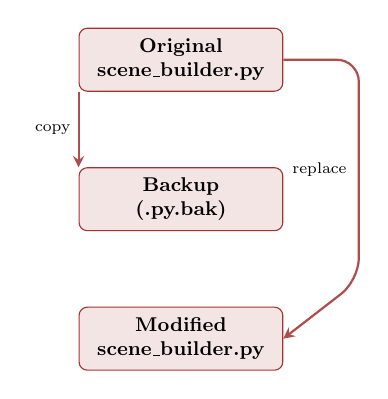
\begin{tikzpicture}[scale=0.8, transform shape, node distance=1.2cm]
        % Nodes
        \node[module, text width=3cm] (original) {Original\\scene\_builder.py};
        \node[module, text width=3cm, below=of original] (backup) {Backup\\(.py.bak)};
        \node[module, text width=3cm, below=of backup] (modified) {Modified\\scene\_builder.py};

        % Copy arrow (left side)
        \draw[arrow] (original.south west) -- node[left] {\scriptsize copy} (backup.north west);

        % Replace arrow (right side, curved)
        \draw[arrow, rounded corners=8pt] (original.east) -- ++(1.2,0) -- ++(0,-3.5) -- (modified.east);
        \node at (2.2,-1.75) {\scriptsize replace};
    \end{tikzpicture}
\end{column}
\end{columns}
\end{frame}

\begin{frame}[fragile]{Scene Builder Update}
\begin{lstlisting}[basicstyle=\ttfamily\scriptsize]
# install.py - Scene builder update
scene_builder_src = script_dir / "scene_builder" / "replicacad" / "scene_builder.py"
scene_builder_dst = maniskill_path / "utils" / "scene_builder" / "replicacad" / "scene_builder.py"

if scene_builder_src.exists() and scene_builder_dst.exists():
    # Backup original
    backup = scene_builder_dst.with_suffix(".py.bak")
    if not backup.exists():
        shutil.copy2(scene_builder_dst, backup)
        print(f"Backed up original to {backup.name}")

    # Replace with modified version
    shutil.copy2(scene_builder_src, scene_builder_dst)
    print(f"Updated scene_builder.py")
\end{lstlisting}
\end{frame}

% ============================================
% SECTION 7: VERIFICATION
% ============================================
\section{Verification}

\begin{frame}[fragile]{Verification - Import Check}
\textbf{Step 1: Verify Python Import}

\vspace{0.3cm}

\begin{lstlisting}
python -c "from mani_skill.agents.robots import aloha_mini; print('OK')"
\end{lstlisting}

\vspace{0.5cm}

\textbf{Expected Output:}
\begin{lstlisting}[basicstyle=\ttfamily\small,numbers=none]
OK
\end{lstlisting}

\vspace{0.5cm}

\begin{block}{If ImportError}
ManiSkill not installed or agent not registered.\\
\textbf{Fix:} \code{pip install mani-skill \&\& python install.py}
\end{block}
\end{frame}

\begin{frame}[fragile]{Verification - Run Demo}
\textbf{Step 2: Test Teleoperation Demo}

\vspace{0.3cm}

\begin{lstlisting}
cd maniskill/teleop
python demo_teleop.py --render
\end{lstlisting}

\vspace{0.5cm}

\textbf{Expected Behavior:}
\begin{itemize}
    \item ManiSkill3 viewer window opens
    \item AlohaMini robot visible in scene
    \item Keyboard controls functional (WASD, arrows)
\end{itemize}

\vspace{0.3cm}

\begin{block}{Tip}
Use \code{--help} flag to see all available options.
\end{block}
\end{frame}

\begin{frame}[fragile]{Verification - File Check}
\textbf{Step 3: Verify Installed Files}

\vspace{0.3cm}

\begin{columns}
\begin{column}{0.5\textwidth}
\textbf{Agent Files:}
\begin{lstlisting}[basicstyle=\ttfamily\scriptsize]
ls $(python -c "
import mani_skill
print(mani_skill.__file__.replace(
  '__init__.py',
  'agents/robots/aloha_mini'))")
\end{lstlisting}

\vspace{0.2cm}

\textbf{Expected:}
\begin{itemize}
    \item \code{\_\_init\_\_.py}
    \item \code{base\_agent.py}
    \item \code{aloha\_mini\_so100\_v2.py}
\end{itemize}
\end{column}
\begin{column}{0.5\textwidth}
\textbf{Asset Files:}
\begin{lstlisting}[basicstyle=\ttfamily\scriptsize]
ls ~/.maniskill/data/robots/aloha_mini/
\end{lstlisting}

\vspace{0.2cm}

\textbf{Expected:}
\begin{itemize}
    \item \code{aloha\_mini\_so100.urdf}
    \item \code{so100\_meshes/}
\end{itemize}
\end{column}
\end{columns}
\end{frame}

\begin{frame}{Troubleshooting - Common Errors}
\begin{table}
\centering
\begin{tabular}{p{3.5cm}p{4cm}p{4.5cm}}
\toprule
\textbf{Error} & \textbf{Cause} & \textbf{Solution} \\
\midrule
\textcolor{red}{\texttt{ImportError}} & ManiSkill not installed & \code{pip install mani-skill} \\
\addlinespace
\textcolor{red}{\texttt{FileNotFoundError}} & URDF/mesh missing & Re-run \code{python install.py} \\
\addlinespace
\textcolor{red}{\texttt{ModuleNotFoundError}} & Agent not registered & Check \code{\_\_init\_\_.py} imports \\
\bottomrule
\end{tabular}
\end{table}

\vspace{0.5cm}

\begin{block}{Debugging Tip}
Run with verbose flag for detailed output: \code{python install.py --verbose}
\end{block}
\end{frame}

\begin{frame}[fragile]{Troubleshooting - Quick Fixes}
\begin{columns}
\begin{column}{0.5\textwidth}
    \textbf{Complete Reinstall:}
\begin{lstlisting}[basicstyle=\ttfamily\scriptsize,numbers=none]
python install.py --uninstall
python install.py
\end{lstlisting}

    \vspace{0.3cm}

    \textbf{Check ManiSkill Version:}
\begin{lstlisting}[basicstyle=\ttfamily\scriptsize,numbers=none]
python -c "import mani_skill; print(mani_skill.__version__)"
\end{lstlisting}
\end{column}
\begin{column}{0.5\textwidth}
    \textbf{Verify Paths:}
\begin{lstlisting}[basicstyle=\ttfamily\scriptsize,numbers=none]
python -c "import mani_skill; print(mani_skill.__file__)"
\end{lstlisting}

    \vspace{0.3cm}

    \textbf{Check Data Directory:}
\begin{lstlisting}[basicstyle=\ttfamily\scriptsize,numbers=none]
ls -la ~/.maniskill/data/robots/
\end{lstlisting}
\end{column}
\end{columns}
\end{frame}

% ============================================
% SECTION 8: UNINSTALLATION
% ============================================
\section{Uninstallation}

\begin{frame}[fragile]{Uninstallation - Command}
\textbf{Remove AlohaMini from ManiSkill}

\vspace{0.5cm}

\begin{lstlisting}
python install.py --uninstall
\end{lstlisting}

\vspace{0.5cm}

\textbf{What Gets Removed:}
\begin{itemize}
    \item \textbf{Agent Files:} \code{mani\_skill/agents/robots/aloha\_mini/}
    \item \textbf{Asset Files:} \code{\textasciitilde/.maniskill/data/robots/aloha\_mini/}
    \item \textbf{Scene Builder:} Restores original from \code{.py.bak} backup
\end{itemize}

\vspace{0.3cm}

\begin{block}{Safe Operation}
Original \code{scene\_builder.py} is restored from backup created during installation.
\end{block}
\end{frame}

\begin{frame}[fragile]{Uninstallation - Code}
\begin{lstlisting}
def uninstall():
    maniskill_path = find_maniskill_path()
    data_dir = get_maniskill_data_dir()

    # Remove agent files
    agent_dst = maniskill_path / "agents" / "robots" / "aloha_mini"
    if agent_dst.exists():
        shutil.rmtree(agent_dst)

    # Remove asset files
    asset_dst = data_dir / "robots" / "aloha_mini"
    if asset_dst.exists():
        shutil.rmtree(asset_dst)

    # Restore scene builder backup
    backup = scene_builder_dst.with_suffix(".py.bak")
    if backup.exists():
        shutil.copy2(backup, scene_builder_dst)
        backup.unlink()  # Remove backup file
\end{lstlisting}
\end{frame}

% ============================================
% SUMMARY
% ============================================

\begin{frame}{Summary}
\centering
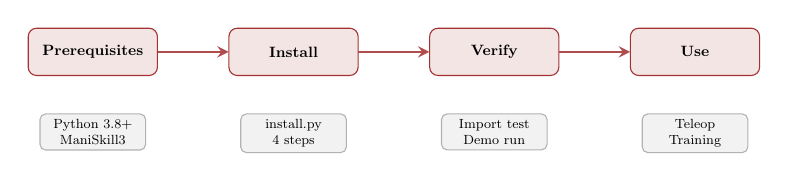
\begin{tikzpicture}[scale=0.6, transform shape, node distance=1.5cm]
    % Main flow
    \node[module, text width=2.5cm] (prereq) {Prerequisites};
    \node[module, text width=2.5cm, right=of prereq] (install) {Install};
    \node[module, text width=2.5cm, right=of install] (verify) {Verify};
    \node[module, text width=2.5cm, right=of verify] (use) {Use};

    \draw[arrow] (prereq) -- (install);
    \draw[arrow] (install) -- (verify);
    \draw[arrow] (verify) -- (use);

    % Details
    \node[submodule, text width=2cm, below=0.8cm of prereq] {Python 3.8+\\ManiSkill3};
    \node[submodule, text width=2cm, below=0.8cm of install] {install.py\\4 steps};
    \node[submodule, text width=2cm, below=0.8cm of verify] {Import test\\Demo run};
    \node[submodule, text width=2cm, below=0.8cm of use] {Teleop\\Training};
\end{tikzpicture}

\vspace{1cm}

\begin{block}{Quick Start}
\centering
\code{pip install mani-skill \&\& python install.py \&\& python demo\_teleop.py}
\end{block}
\end{frame}

% Final slide
\begin{frame}
\centering
\vspace{2cm}
{\Huge\color{darkred} Setup Complete}

\vspace{1cm}

{\large ManiSkill3 + AlohaMini Integration}

\vspace{0.5cm}

Robot UID: \code{aloha\_mini\_so100\_v2}
\end{frame}

\end{document}
